\chapter{Introduzione}


    % INTERFACCIA GRAFICA
    \section{Interfaccia grafica}

        \begin{notebox}
            Tutte le seguenti sotto-finestre possono essere spostate, affiancate, ingrandite o rimpicciolite.

            Per ritornare al layout di default delle finestre andare su window, load layout, load default layout.
        \end{notebox}

        \begin{notebox}
            Premendo F10 si entra nella "Docked mode" che nasconde tutte le sotto-finestre nella sidebar.
        \end{notebox}


        % VIEWPORT
        \subsection{Viewport}
            La viewport e' la finestra principale (figura \ref{fig:unreal_editor}) e permette di inserire, muovere e modificare gli oggetti e di muoversi nel mondo di gioco.

            Per muoversi all'interno della viewport occorre tenere premuto il tasto destro e cliccare i tasti W (avanti), A (sinistra), S (indietro), D (destra).
            Per muoversi verticalmente bisogna premere il tasto E (verso l'alto) o il tasto Q (verso il basso).

            Cliccando sul simbolo della telecamera \UECameraIcon e' possibile aumentare o diminuire la velocita' del movimento.

            \begin{notebox}
                E' anche possibile modificare la velocita' dei movimenti tenendo premuto il tasto destro della viewport e ruotando la rotellina del mouse.
            \end{notebox}

            Per teletrasportarsi vicino ad un oggetto si puo' selezionarlo dall'outliner (si trova in alto a destra del viewport) e poi premere il tasto F. (Focus)

            Dopo aver selezionato e aver fatto il focus su un oggetto e' possibile:
            \begin{itemize}
                \item Eseguire lo zoom sull'oggetto tenendo premuto il tasto ALT e il tasto destro del mouse e muovendo fisicamente il mouse avanti e indietro oppure ruotando la rotellina.
                \item Ruotare la visuale attorno all'oggetto tenendo premuto il tasto ALT e il tasto sinistro del mouse e muovendo fisicamente il mouse.
            \end{itemize}

            In alto a sinistra, all'interno della viewport, e' presente il tasto "Perspective" \UEPerspectiveIcon che permette di cambiare prospettiva (ad esempio visualizzare gli oggetti dall'alto).

            \begin{notebox}
                Per muoversi dalla prospettiva dall'alto bisogna cliccare il pulsante destro del mouse e trascinarlo. La rotellina del mouse permette di eseguire uno zoom.
            \end{notebox}

            Per tornare alla modalita' "Perspective" e' possibile farlo dal tasto di prima oppure premere ALT + G.

            Di fianco al tasto "Perspective" e' presente il tasto per modificare la "View mode" \UEViewModeIcon con cui e' possibile vedere il mondo di gioco:
            \begin{itemize}
                \item "Lit": con illuminazione del mondo di gioco
                \item "Unlit": senza illuminazione (illuminazione "costante" ovunque che permette di vedere i colori "naturali" degli oggetti)
                \item "Wireframe": permette di vedere spigoli e angoli degli oggetti
                \item \dots
            \end{itemize}

            Di fianco al tasto per modificare la "View mode" e' presente il tasto per visualizzare le "Show flags" (figura \ref{fig:unreal_editor_show_btn}): permettono di attivare o disattivare certe tipologie di oggetti.

            \begin{notebox}
                Cliccando su "Use defaults" verranno reimpostate le flag originali.
            \end{notebox}

            A sinistra del pulsante "Perspective" c'e' un pulsante hamburger da cui si puo' visualizzare la "Game view" (attivabile con il pulsante G). La "Game view" permette di visualizzare direttamente nell'editor il mondo di gioco con gli occhi del giocatore.

            \begin{notebox}
                L'hotkey per passare in questa modalita' e' il tasto G.
            \end{notebox}

            Con CTRL + L si puo' spostare il sole per vedere i riflessi della luce da varie angolazioni su un oggetto.


            \subsubsection{Spostare, ruotare e traslare gli oggetti}


                Per spostare gli oggetti bisogna selezionare in alto a destra il pulsante \UEMovementEditingIcon a destra del pulsante con il cursore. A quel punto e' possibile utilizzare gli assi di traslazione/spostamento (chiamato "gizmo" in Unreal Engine) dell'oggetto selezionato per spostarlo lungo un certo asse.

                \begin{notebox}
                    E' possibile spostare l'oggetto in modo fluido disattivando la funzione "snap" cliccando sul pulsante griglia \UEGridSnappingIcon oppure attivarlo per effettuare spostamenti lungo una griglia.

                    E' anche possibile modificare la dimensione della griglia per fare spostamenti piu' o meno precisi (l'unita' di misura e' in centimetri).
                \end{notebox}

                Cliccando il cubo al centro dei 3 assi sull'oggetto e' possibile spostare l'oggetto lungo tutte le direzioni.

                \begin{notebox}
                    Tenendo premuto il tasto shift fa in modo che la telecamera segua l'oggetto che stiamo spostando.
                \end{notebox}

                \begin{notebox}
                    Premendo sulla tastiera il tasto "Fine" oppure "End" e' possibile far appoggiare un oggetto sulla superficie che si trova al di sotto dell'oggetto stesso.
                \end{notebox}

                Per ruotare gli oggetti bisogna selezionare il pulsante di rotazione \UEMovementEditingIcon a destra del pulsante di movimentazione degli oggetti. Utilizzando gli assi e' possibile ruotare l'oggetto.

                \begin{notebox}
                    Anche la rotazione ha il pulsante per attivare o disattivare la griglia \UERotationSnappingIcon (ed e' possibile modificare la precisione).
                \end{notebox}

                Per ridimensionare gli oggetti e' presente il pulsante relativo a destra del pulsante di rotazione \UEMovementEditingIcon. Anche in questo caso e' possibile operare lungo uno dei 3 assi per ridimensionare l'oggetto lungo quella dimensione.

                \begin{notebox}
                    Anche il ridimensionamento puo' essere fatto lungo una scala di fattori distanzati equivalentemente oppure no cliccando il pulsante relativo \UEScaleSnappingIcon.
                \end{notebox}

                Cliccando il cubo al centro dei 3 assi e' possibile ridimensionare l'oggetto in modo uniforme lungo tutte le dimensioni.

                Tutte e 3 le operazioni possono essere effettuate relativamente all'oggetto stesso oppure relativamente ad un asse globale.
                (Cliccando sul tasto con il globo \UEGlobalIcon a destra del pulsante \UEMovementEditingIcon o cubo a seconda del punto di riferimento attuale)

            \subsubsection{Creare un oggetto}
                Cliccare il tasto "add" \UEQuickAddIcon nella toolbar e da li e' possibile aggiungere:
                \begin{itemize}
                    \item Una shape
                    \item Una luce
                    \item \dots
                \end{itemize}

                Un'altra alternativa e' andare nel content browser/drawer (che si apre premendo il tasto relativo \UEContentBrowserIcon in basso a sinistra), selezionare un oggetto e trascinarlo nella viewport.

            \subsubsection{Duplicare gli oggetti}

                Per duplicare un oggetto e' possibile:
                \begin{itemize}
                    \item Cliccare CTRL + D (Duplicate) e poi spostare la copia (l'oggetto copia e l'originale sono sovrapposti).
                    \item Tenere premuto il tasto ALT e contemporaneamente spostare l'oggetto manterra' l'oggetto originale nella sua posizione e spostera' una copia.
                \end{itemize}

            \subsubsection{Selezionare piu' oggetti}
                Tenendo premuto shift e' possibile cliccare sugli oggetti per selezionarli tutti.

                Per de-selezionare un oggetto bisogna tener premuto CTRL e cliccare sull'oggetto da rimuovere.

            \subsubsection{Cancellare uno o piu' oggetti}
                Per cancellare un oggetto e' sufficiente selezionarlo e premere il tasto "Del" oppure "Canc".

                Per cancellare piu' oggetti bisogna prima selezionare tutti gli oggetti da cancellare utilizzando shift per selezionare dall'outliner un insieme di oggetti adiacenti oppure tenendo premuto il tasto CTRL e cliccando i singoli oggetti (dalla viewport oppure dall'outliner) che si vuole selezionare.

        \subsection{Toolbar}
            Nella toolbar sono presenti diversi tasti, tra cui:
            \begin{itemize}
                \item Il pulsante "add" \UEQuickAddIcon: permette di aggiungere oggetti nel mondo di gioco.
                \item Il menu' a tendina per selezionare la modalita' tra cui:
                    \begin{itemize}
                        \item La "Select Mode": permette di selezionare, spostare e ridimensionare oggetti
                        \item La "Landscape Mode": permette di creare una landscape
                        \item La "Foliage Mode": permette di creare fogliame (bisogna avere gli asset disponibili per poter piazzare il fogliame)
                    \end{itemize}
            \end{itemize}

            La toolbar e' posizionata sopra alla viewport.

        \subsection{Outliner panel}
            E' una lista gerarchica di tutti gli oggetti che appartengono al mondo di gioco. E' posizionata a destra della viewport (in alto).

            Si possono selezionare gli oggetti cliccando sull'oggetto nella viewport oppure cliccando sull'oggetto dall'Outliner. E' possibile tenere premuto il tasto CTRL per selezionare piu' oggetti.

            Per organizzare gli oggetti si puo' cliccare il tasto destro nell'outliner e selezionare "Create folder" per creare una cartella e poi trascinare gli oggetti al suo interno.

            E' anche possibile nascondere temporaneamente gli oggetti cliccando sull'occhio a sinistra dell'oggetto da nascondere. Cliccare di nuovo l'occhio (chiuso) fara' riapparire l'oggetto.

        \subsection{Details panel}
            Permette di modificare le proprieta' dell'oggetto selezionato. E' posizionato sotto all'outliner e a destra del viewport (in basso).

            Ogni modifica puo' essere annulata premendo CTRL+Z.

            \begin{notebox}
                A destra di ogni impostazione modificata e' presente una freccia che permette di resettare l'impostazione al valore di default.
            \end{notebox}

        \subsection{Content Browser/Drawer}
            Contiene tutte le informazioni degli oggetti e del mondo di gioco. Per farlo apparire bisogna cliccare il pulsante in basso a sinistra \UEContentBrowserIcon chiamato "Content drawer" oppure premere CTRL + barra spaziatrice.

            Tutto e' contenuto in sotto-cartelle navigabili facendo doppio click.

            E' possibile aprire un asset facendo doppio click sull'asset. Se si fa questa operazione su:

            \begin{itemize}
                \item Una mesh: viene aperto il "static mesh editor" che permette di modificare l'asset.
                \item Una mappa: viene aperta la mappa. (Verra' chiesto se salvare o eliminare le modifiche effettuate sulla mappa corrente)
            \end{itemize}

            Il pulsante "Add" in alto a sinistra all'interno del content drawer permette ad esempio di:
            \begin{itemize}
                \item Cliccare su "Add feature or content pack" per aggiungere nuovi contenuti tra cui il "Starter content" (gli oggetti iniziali)
            \end{itemize}

            Premendo il tasto "Dock in Layout" in alto a destra nel content drawer permette di tenere sempre aperto il content drawer.

            Cliccando il pulsante "Settings", a destra di "Dock in Layout", e' possibile attivare "Show Engine Content" per far apparire nel "Content browser" una cartella contenente tutti gli oggetti di default di Unreal Engine.

            Premendo il tasto destro e' possibile:
            \begin{itemize}
                \item Creare una nuova cartella cliccando su "new folder"
                \item Importare asset cliccando su "import to game"
                \item Aggiungere modelli e texture da quixel bridge cliccando su "add quixel content"
            \end{itemize}

            \begin{figure}[h]
                \caption{Unreal Engine: Content Browser}
                \centering
                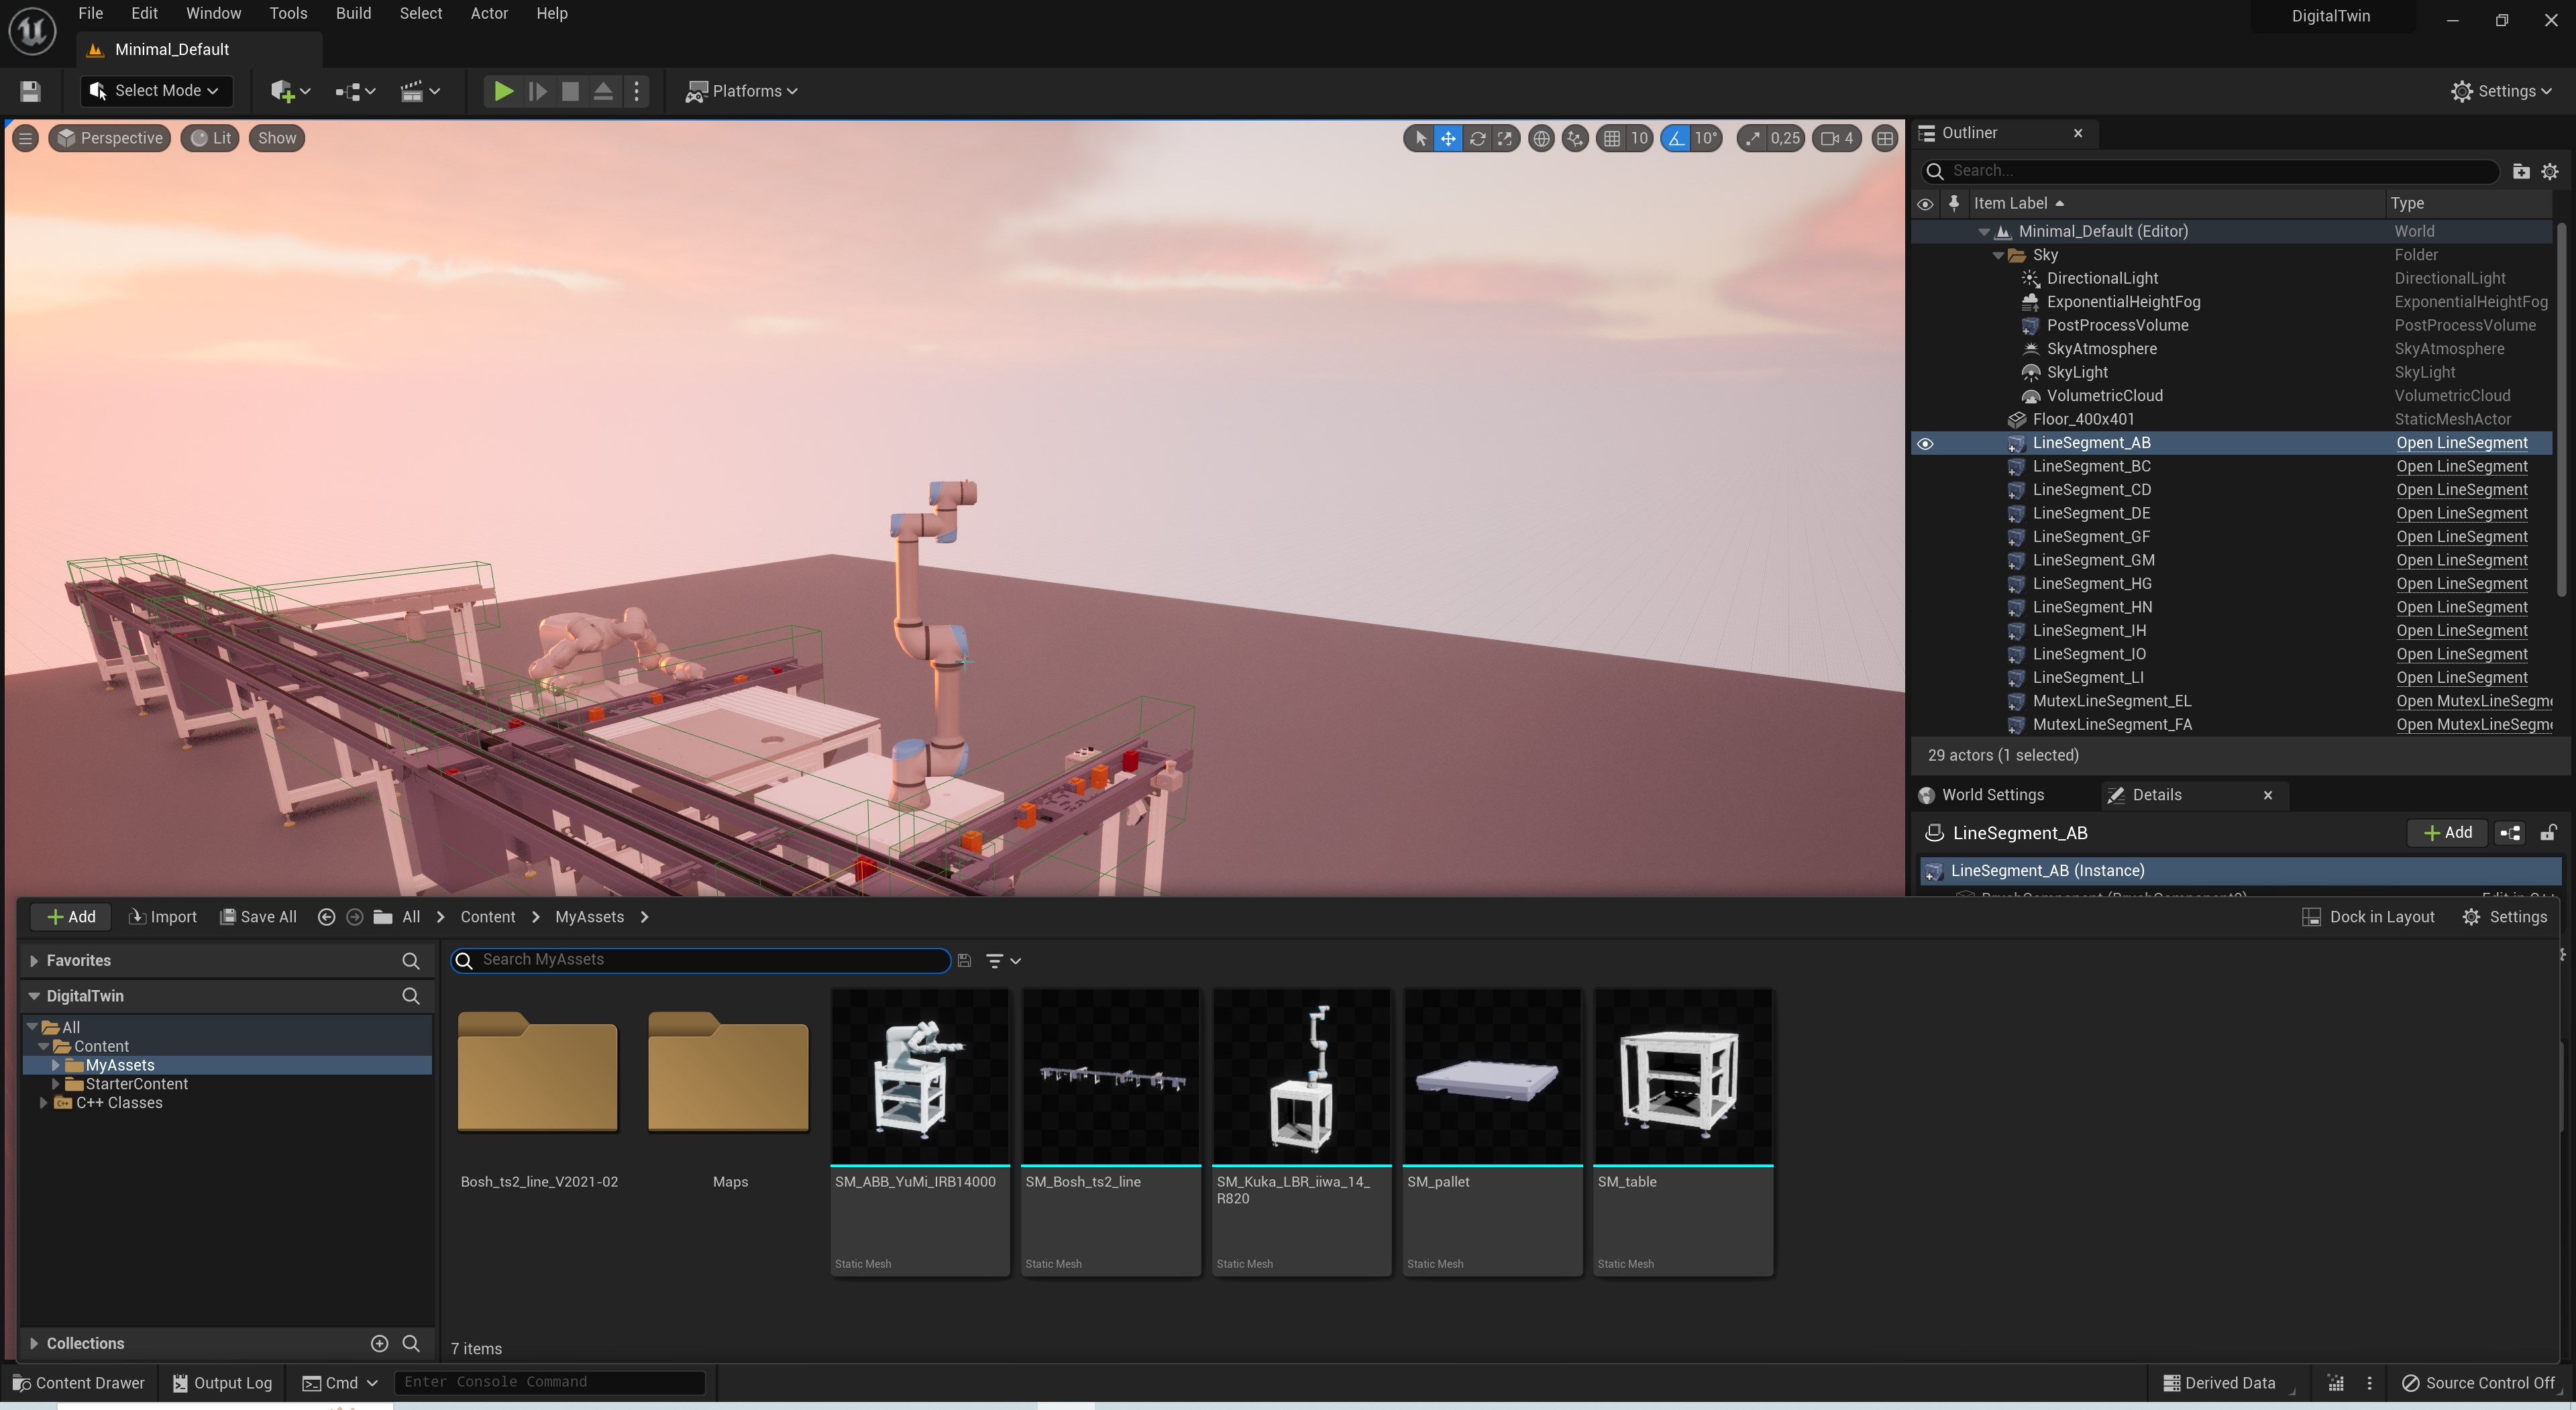
\includegraphics[width=\textwidth]{unreal_engine-content_browser}
                \label{fig:unreal_engine_content_browser}
            \end{figure}

        \subsection{Menu Bar}
            La "Menu Bar" e' la barra in alto di fianco al logo di unreal engine.

            La "Menu Bar permette:
            \begin{itemize}
                \item Cliccando su "Window" di vedere una lista di tutte le finestre.

                    Tra le finestre presenti sotto a "Window" troviamo:
                    \begin{itemize}
                        \item "World Settings": permette di modificare delle impostazioni della mappa aperta.
                        \item "Load Layout": permette di impostare le sotto-finestre secondo un certo layout.

                                L'impostazione "Default Editor Layout" permette di ritornare al layout originale.

                    \end{itemize}
            \end{itemize}


        %FIGURE

        \begin{figure}[h]
            \caption{Unreal Engine: Unreal Editor}
            \centering
            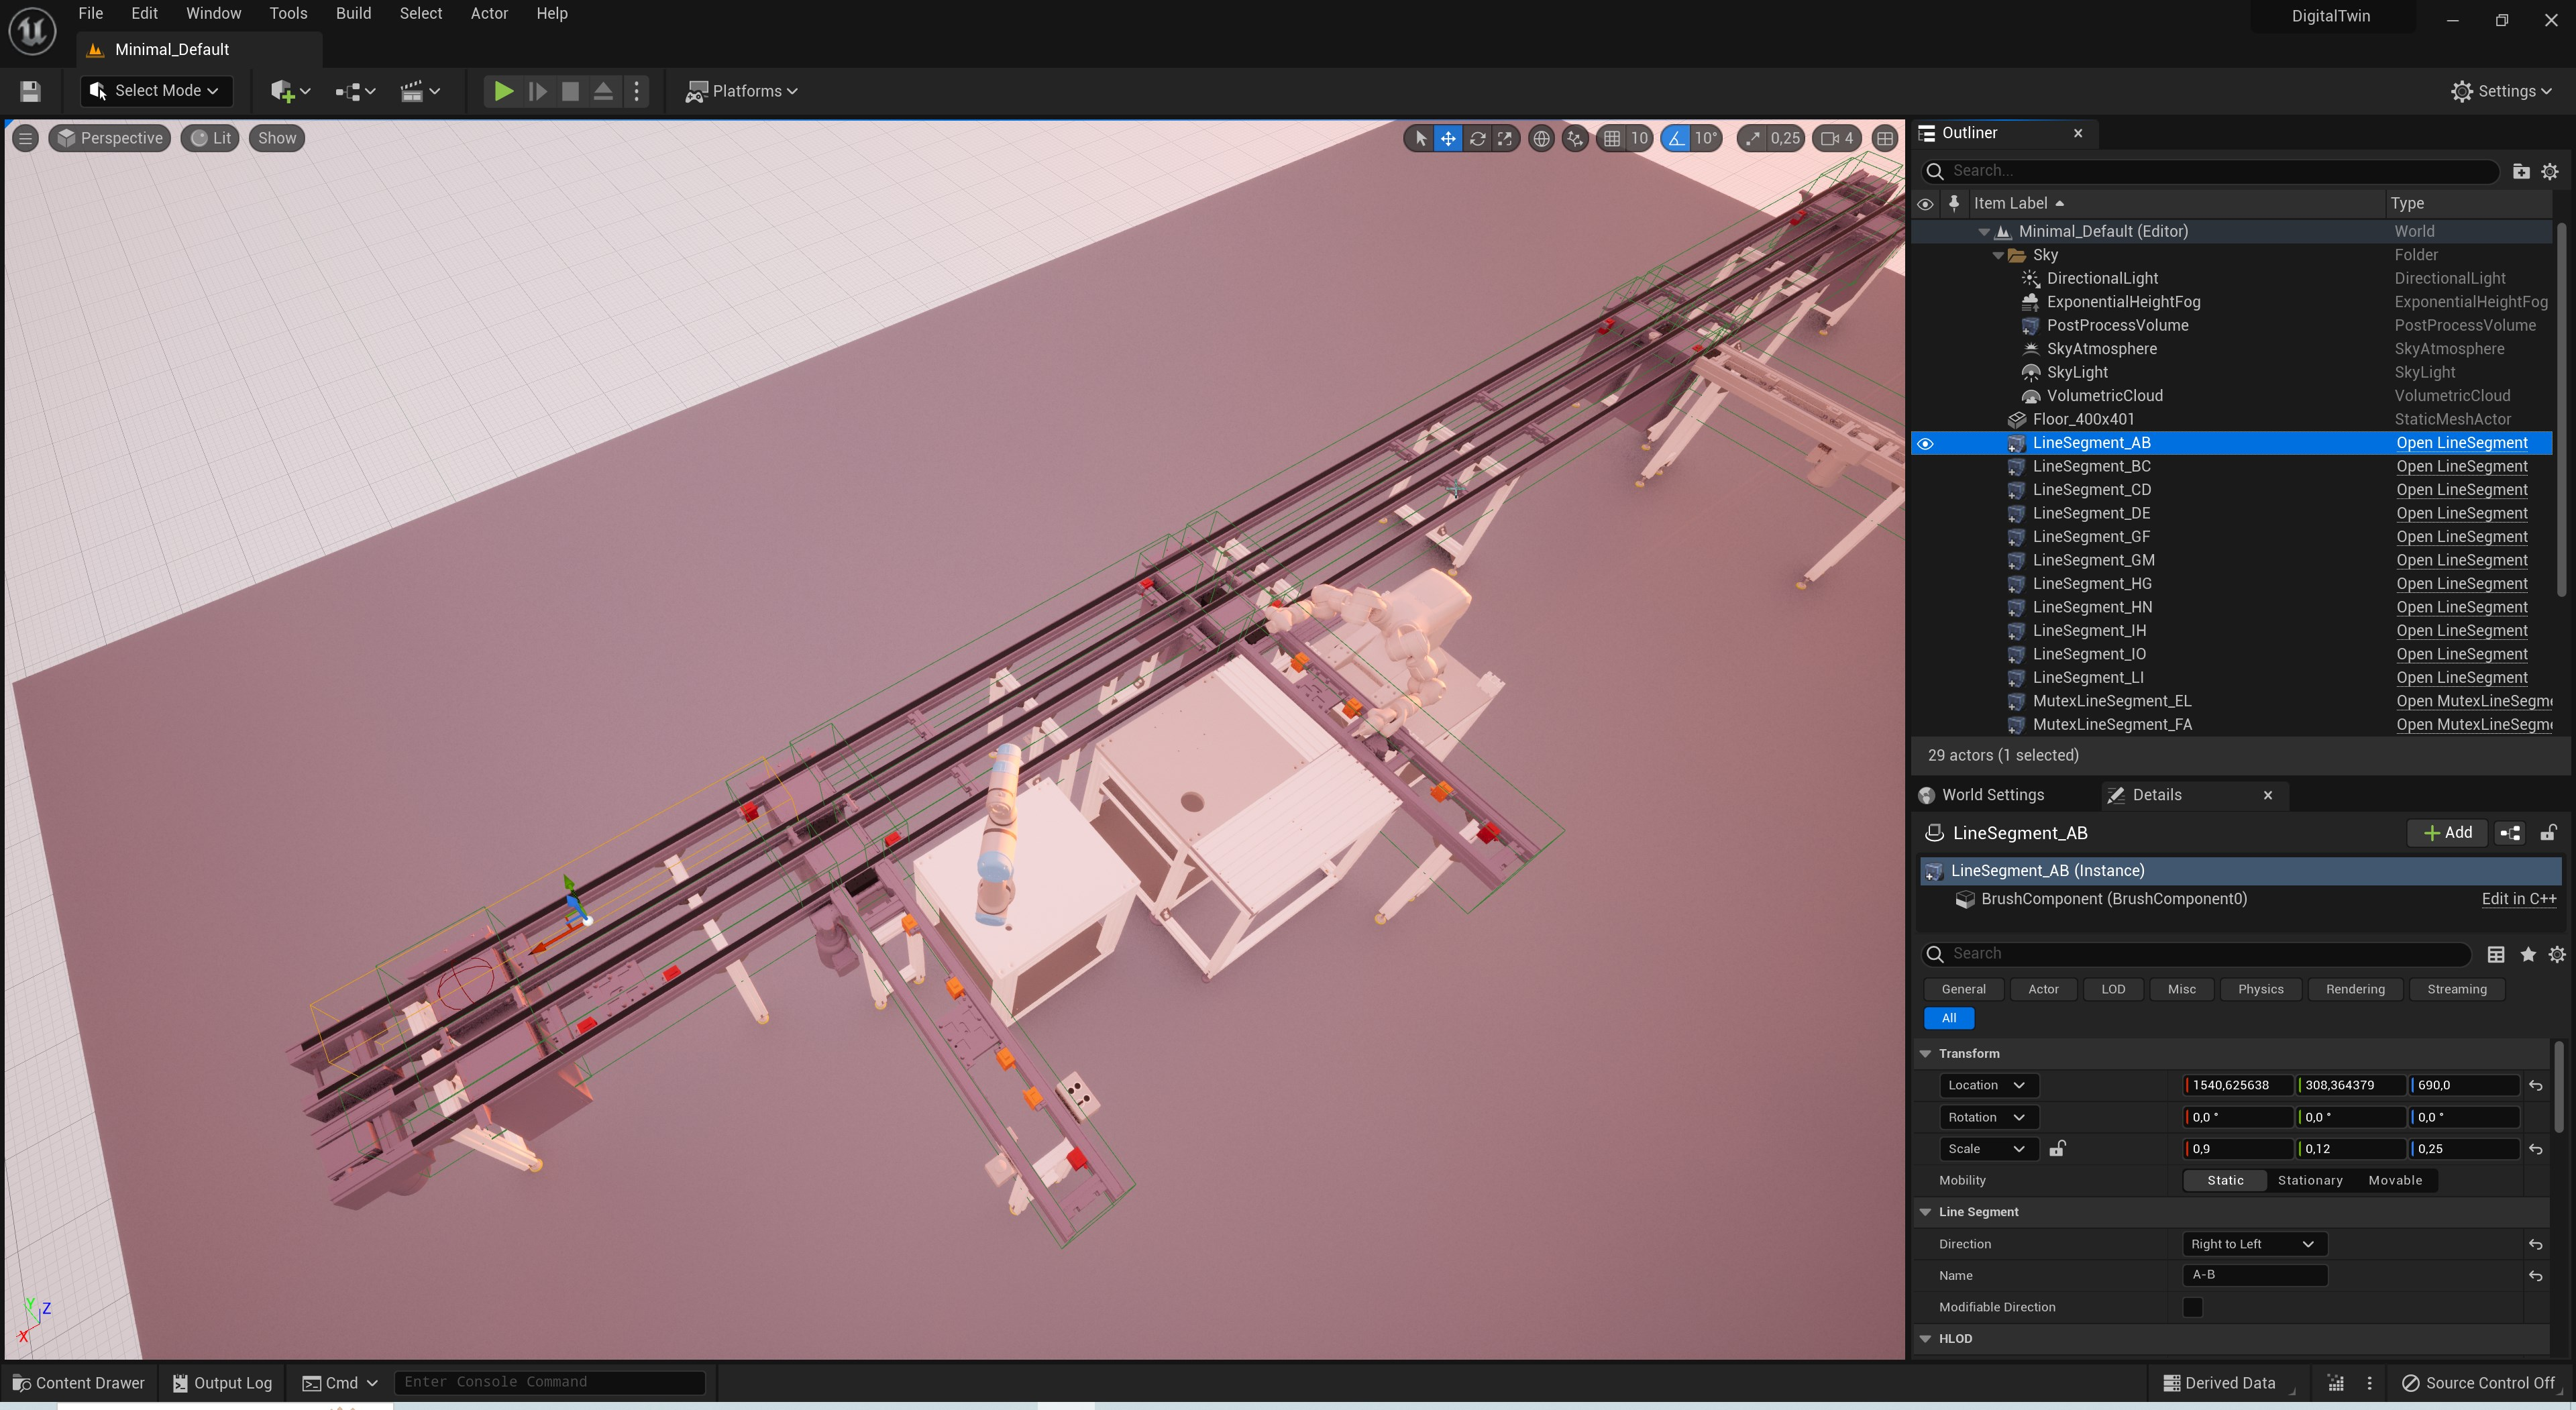
\includegraphics[width=\textwidth]{unreal_editor}
            \label{fig:unreal_editor}
        \end{figure}

        \begin{figure}[h]
            \caption{Unreal Engine: Unreal Editor Show flags}
            \centering
            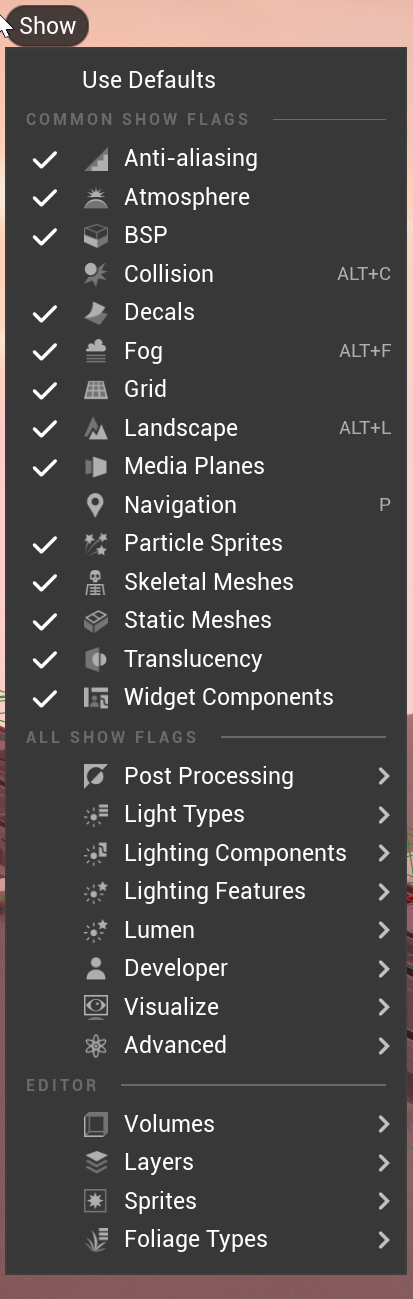
\includegraphics[height=500pt]{unreal_editor-show_btn}
            \label{fig:unreal_editor_show_btn}
        \end{figure}

    % POST-PROCESSING
    \section{Post-Processing}

        \subsection{Auto-exposure}
            Di default Unreal Engine simula l'adattamento degli occhi alla luce e all'ombra modificando la luminosita'.

            Per disattivarlo nell'editor e' possibile cliccare sul pulsante "Lit" e de-selezionare "Game settings" sotto a "Exposure".

            Sempre all'interno di quel menu' a tendina e' possibile modificare "EV100" per modificare la luminosita'.

            Per disattivare l'auto-exposure nel gioco bisogna selezionare l'oggetto "GlobalPostProcessVolume" dall'outliner e poi andare nel "Details panel" e modificare l'impostazione  "exposure compensation" dopo aver attivato e impostato l'opzione "Metering Mode" a "Manual".


        % POSTPROCESSVOLUME
        \subsection{PostProcessVolume}
            I "PostProcessVolume" permettono di aggiungere degli effetti visivi dopo il rendering. Questi effetti influiscono sulla telecamera e non sul mondo di gioco.

            Per creare un PostProcessVolume bisogna andare in "add" nella toolbar, selezionare "volumes" e poi "PostProcessVolume".

            Esempio di impostazioni:
            \begin{itemize}
                \item Vignette Intensity: permette di scurire i bordi dello schermo
                \item (Bloom) Intensity: intensita' dei raggi di luce
                \item (Color Grading - Global) Saturation

                    \begin{notebox}
                        Impostando la saturazione a zero e' possibile rendere tutto bianco e nero.
                    \end{notebox}

                \item \dots
            \end{itemize}

            Di default un "PostProcessVolume" ha effetto solo all'interno della sua area. Per rendere l'effetto globale bisogna selezionare l'opzione "Infinite Extent (Unbound)".

            \begin{notebox}
                Per vedere l'effetto del "PostProcessVolume" occorre andare sul pulsante "Lit"/"Unlit" e selezionare l'opzione "Game settings"
            \end{notebox}


    % CREARE UN NUOVO LIVELLO
    \section{Creare un nuovo livello}
        Per creare un nuovo livello e' possibile:
        \begin{itemize}
            \item Andare nel content drawer, fare click con il tasto destro e selezionare "Level" sotto a "Create basic asset".

                \begin{notebox}
                    Il livello sara' vuoto
                \end{notebox}

            \item Andare su "File", "New level" e selezionare un template predefinito.
        \end{itemize}


    % CREARE UN PUNTO DI SPAWN
    \section{Creare un punto di spawn}
        Per definire un punto di spawn bisogna cliccare su "add", "all classes", "player start".

        Se appare l'errore "bad size" significa che il player start collide con un oggetto e che e' necessario spostarlo.

        Dopo aver selezionato il player start, premendo il tasto "end"/"fine" della tastiera, e' possibile posizionare il punto di spawn sull'oggetto immediatamente sotto di esso.

        Vicino al triangolo verde per iniziare il gioco e' possibile impostare con i 3 puntini verticali il punto di spawn come "default player start".


    % INTRODUZIONE AI MATERIALI
    \section{Introduzione ai materiali}

        \subsection{Utilizzare un materiale}
            Per utilizzare un materiale e' sufficiente selezionarlo nel Content Browser e trascinarlo sull'oggetto che deve essere fatto del materiale desiderato.

            \begin{notebox}
                Per rendere effettive le modifiche effettuate su un materiale utilizzando il Material Editor bisogna compilare il materiale.
            \end{notebox}

        \subsection{Creare un materiale}

            Per creare un materiale occorre:
            \begin{enumerate}
                \item Cliccare il tasto destro in una cartella del content browser
                \item Selezionare sotto alla categoria "Create basic asset" la voce "Material"
                \item Dare un nome al materiale

                    \begin{notebox}
                        Tipicamente un materiale ha il nome che inizia con "M\_"
                    \end{notebox}

            \end{enumerate}

            Facendo doppio click su un materiale e' possibile aprire il "Material editor" che permette di personalizzare il materiale.

            \begin{notebox}
                Tenendo premuto il tasto sinistro sulla finestra del "Material editor" e' possibile spostarla e posizionarla di fianco alla tab del livello.

                In questo modo, al posto di avere due finestre separate, si avranno due tab come accade nei browser.
            \end{notebox}

        \subsection{Material Editor}

            Il material editor serve per creare o personalizzare un materiale.

            Per modificare un materiale e' possibile fare doppio click sul materiale che si trova nel content drawer oppure selezionando un oggetto e' possibile vedere nel details panel i materiali che compongono l'oggetto. Facendo doppio click su uno dei materiali che compone l'oggetto si aprira' il Material Editor.

            \begin{notebox}
                E' anche possibile cliccare il pulsante vicino al materiale dal details panel per aprire il content browser nella cartella contenente il materiale e poi fare doppio click sul materiale stesso.
            \end{notebox}

            Il Material Editor e' composto da:
            \begin{itemize}
                \item Il "Material Graph": e' formato da nodi interconnessi che permettono di creare il materiale desiderato.

                    Il nodo di default e' il nodo finale di una catena di nodi.

                \item La "Viewport" permette di vedere un'anteprima del materiale.

                    In basso e' possibile decidere se visualizzare il materiale su un modello a forma di cilindro, su una sfera, su un cubo o su una superficie.

                \item Il "Details Panel" permette di modificare le proprieta' del nodo selezionato.

                \item La "Palette" (pulsante a destra del material graph) permette di trovare tutti i tipi di nodi inseribili nel Material graph.

                    \begin{notebox}
                        E' anche possibile aprire la "Palette" cliccando il tasto destro nel material graph.
                    \end{notebox}

            \end{itemize}

            I movimenti possibili all'interno del material graph sono:
            \begin{itemize}
                \item Tenendo premuto il tasto destro e muovendo il mouse e' possibile trascinare il grafo per spostarsi
                \item La rotellina del mouse permette di eseguire lo zoom
                \item Cliccare un nodo permette di selezionarlo
                \item Tenendo premuto il tasto sinistro e muovendo il mouse e' possibile selezionare piu' nodi contemporaneamente
                \item Tenendo premuto il tasto ALT e cliccando su un punto di giunzione di un filo (pin) con il tasto sinistro permette di cancellare quel filo.
                \item Tenendo premuto il tasto CTRL e cliccando su un punto di giunzione di un filo (pin) con il tasto sinistro del mouse permette di spostare il filo da un input/output ad un altro.
            \end{itemize}

            Tra i nodi presenti nella "Palette" troviamo:
            \begin{itemize}
                \item "Constant3Vector": e' un colore selezionabile dai parametri RGB.

                    Per applicare il colore costante e' sufficiente collegare il nodo Constant3Vector con il nodo finale nell'uscita chiamata "Base Color".

                \item "Constant": e' un valore costante.

                    E' utile ad esempio per impostare se un oggetto e' liscio oppure ruvido collegando il nodo all'output "Roughness". Impostando questo valore vicino a zero si ottiene un materiale riflettente.

                    \begin{notebox}
                        Roughness deve essere un valore tra zero e uno. Zero significa liscio e uno significa ruvido.
                    \end{notebox}

                    Un'altro esempio potrebbe essere impostare l'opzione "Metallic" per rendere l'oggetto metallico o meno.

                    \begin{notebox}
                        Metallic deve essere un valore tra zero e uno. Uno significa metallico.
                    \end{notebox}

                \item "Texture Sample": permette di aggiungere una texture all'oggetto.

                    Un utilizzo pratico delle texture e' rendere imperfetta la superficie di un oggetto impostando nel details panel l'opzione "Texture" a "T\_Perlin\_Noise\_M" e collegando il valore "RGB" a "Roughness.

                    \begin{notebox}
                        La texture contiene pixel aventi valori tra zero e uno.
                    \end{notebox}

                \item "Linear Interpolate": permette di utilizzare un colore sotto certe condizioni oppure un'altro colore in altre.

                    Ad esempio e' possibile collegare due colori diversi agli input "A" e "B" e collegare all'input "Alpha" l'output "RGB" di una texture:
                    in questo modo alcune aree saranno colorate del primo colore e le altre nel secondo colore.

                    \begin{notebox}
                        Utile ad esempio per far sembrare sporche alcune superfici.
                    \end{notebox}

                    E' anche possibile utilizzare questo nodo per applicare un colore o una texture.
                    Utile ad esempio per applicare la ruggine con la texture "T\_Metal\_Rust\_D".

                    \begin{notebox}
                        E' possibile aprire la texture facendo doppio click su di essa. Se sembra vuota occorre disattivare l'opacita' cliccando sulla "A".
                    \end{notebox}

                \item "Texture Coordinate": permette di scalare una texture attraverso un nodo "Multiply".

                    La texture coordinate va collegata all'input "A" e un valore costante va collegato all'input "B" di "Multiply".

                \item "Multiply": permette di moltiplicare due valori tra di loro.

                \item "Flatten Normal": permette di modificare l'intensita' di una "Normal Map".

                    \begin{notebox}
                        La normal map simula le ombre e le profondita' all'interno dei materiali.
                    \end{notebox}

                \item "StaticSwitchParameter": permette di creare una checkbox che connette un nodo "A" ad un nodo "C" se c'e' la spunta oppure connette il nodo "B" al nodo "C" se non c'e' la spunta.

                    \begin{notebox}
                        True indica che la spunta e' presente, False indica che non e' presenta la spunta.
                    \end{notebox}

            \end{itemize}

            E' anche possibile importare direttamente le texture trascinandole dal content browser nel material graph.

            \begin{notebox}
                E' utile ad esempio per dare una superficie imperfetta ad un materiale (texture "T\_Perlin\_Noise\_M").
            \end{notebox}

            \begin{notebox}
                Per rendere effettive le modifiche effettuate su un materiale utilizzando il Material Editor bisogna compilare il materiale. Per compilare il materiale e' sufficiente cliccare il pulsante "Apply" nella toolbar all'interno del Material editor.
            \end{notebox}

        \subsection{Parametri e istanze dei materiali}
            I parametri permettono di fare modifiche ai materiali senza doverli ricompilare.

            Questo permette di risparmiare molto tempo perche' quando un materiale e' estremamente complesso i tempi di compilazione sono lunghi.

            Per utilizzare i parametri occorre creare un'istanza dei materiali. Per farlo e' sufficiente aprire il content browser e cercare il materiale, cliccare il tasto destro sul materiale e poi cliccare su "Create Material Instance".

            \begin{notebox}
                E' best practice nominare l'istanza come il materiale ma aggiungendo una "I" (Instance) tra la "M" e il "\_": il nome del file iniziera' con "MI\_".
            \end{notebox}

            L'istanza del materiale avra' accesso soltanto ai parametri impostati all'interno del materiale di cui si e' creata l'istanza.

            Per aggiungere parametri al materiale bisogna fare doppio click sul materiale (si aprira' il material editor), fare click con il tasto destro su un nodo da trasformare in parametro e cliccare su "Convert to Parameter".

            Dal "Details panel" dell'istanza del materiale e' possibile modificare i valori dei parametri.

        \subsection{Master Material}
            Un Master Material e' un materiale da cui vengono create istanze molto diverse fra di loro.

            Generalmente un Master Material ha tutti parametri preconfigurati per NON modificare l'aspetto originale delle texture.

            Inoltre anche le texture sono parametri: per convertire una texture in un parametro e' sufficiente cliccare con il tasto destro sulla texture e poi cliccare su "Convert to parameter"

        \subsection{Impostazioni PBR}
            PBR, o Physically Based Rendering, e' la tecnologia che usa Unreal Engine per simulare un materiale.

            Le impostazioni PBR sono:
            \begin{itemize}
                \item Metallic: permette di decidere se e' un materiale plastico (valore vicino a zero) o metallico (valore vicino a 1).
                \item Roughness: permette di decidere se un materiale e' lucido e riflettente (valore vicino a zero) o ruvido (Valore vicino a 1).
            \end{itemize}


    % TEXTURE
    \section{Texture}

        \subsection{Importare una texture}
            Per importare una texture e' sufficiente selezionare i file e trascinarli all'interno del content drawer. I file finiranno nella cartella attualmente aperta nel content drawer.

            Esistono diversi tipi di texture:
            \begin{itemize}
                \item Le "Color texture": contengono il colore
                \item Le "Map"
                \item Le "normalMap": simulano la profondita' dei materiali (esempio cavita' tra i mattoni) e permettono di avere ombra all'interno della texture.

                    \begin{notebox}
                        Nel Material editor bisogna collegare le normal map al nodo finale attraverso l'output "Normal".
                    \end{notebox}
            \end{itemize}

            \begin{notebox}
                Per le "color texture" e' importante assicurarsi che sRGB sia attivo. Per verificare se e' attivo fare doppio click sulla texture e guardare nel details panel. Per le altre texture ("map" e "normalMap") e' meglio disattivare sRGB e assicurarsi che sia selezionato il tipo di texture giusto in "Compression settings".
            \end{notebox}

            \begin{notebox}
                A volte le texture sono separate (un file per metallic, una per roughness, ...) ma potrebbero anche essere condensate in un unico file seguendo canali di colore diversi (red, green, blue). Quando si vogliono utilizzare texture incluse in un unico file bisogna collegare gli output R, G, B divisi al posto di utilizzare l'output singolo "RGB".
            \end{notebox}

            Quando si utilizza una texture in un materiale e' possibile:
            \begin{itemize}
                \item Scalare la texture per uno scalare utilizzando il nodo "Multiply".
                \item Cambiare la tonalita' della texture utilizzando il nodo "Multiply" per moltiplicare la texture per un colore (Constant3Vector).
            \end{itemize}


    % STATIC MESh
    \section{Static Mesh}

        Una static mesh e' un oggetto 3D. Sono composte da vertici, facce e spazio.

        Una static mesh ha un materiale che in genere e' composto da piu' texture.

        \subsection{Importare una static mesh}
            Per importare una static mesh in formato FBX occorre trascinare il file .fbx nel content browser.

            Lasciando i valori di default verra' creato un nuovo materiale. Se si desidera utilizzare un materiale gia' esistente bisogna selezionare nel menu' "Material import Method" il valore "Do Not Create Material".

            I valori di default faranno importare delle texture. Si puo' specificare di non importare le texture per importarle manualmente.


    % ASSET
    \section{Asset}

        \subsection{Migrare asset tra progetti}

            Per spostare un asset da un progetto Unreal Engine ad un altro e' sufficiente andare nel content browser del progetto contenente una cartella da esportare, cliccare sulla cartella con il tasto destro e premere "Migrate".
            A quel punto e' possibile de-selezionare gli asset che non si desidera esportare. Dopo aver cliccato su "OK" verra' chiesto in quale cartella importare i file e cliccare su "Select Folder".

            Il metodo piu' veloce per trovare il percorso e' trovare la cartella nel content drawer nel progetto in cui si desidera IMPORTARE gli asset, fare click con il tasto destro su una cartella e premere "Show in explorer".
            Dopo aver fatto questo basta copiare e incollare il percorso nella finestra di selezione della destinazione dell'export descritta precedente e cliccare su "Select folder".


    % LUMEN: GESTIRE LA LUCE
    \section{Lumen: gestire la luce}

        Lumen permette di gestire in tempo reale l'illuminazione della mappa simulando i riflessi della luce.
        I riflessi contengono parte del colore dell'oggetto riflesso.

        L'impostazione "mobility" permette di scegliere se una luce e' "movable", "stationary" oppure "static":
        \begin{itemize}
            \item static: la luce non cambia a runtime, quindi le ombre e la luce restano fisse. Occorre cliccare su "build > build lighting"
            \item stationary: la luce non si puo' muovere ma le ombre sono dinamiche.
            \item movable: tutto e' dinamico.
        \end{itemize}


        % LUCE STATICA
        \subsection{Luce statica}
            Prima che venisse implementato lumen in Unreal Engine le luci erano sempre statiche.

            \begin{notebox}
                Per disattivare lumen e' possibile andare nel PostProcessVolume e impostare sotto a "Global Illumination", "Method", l'opzione "None"
            \end{notebox}

            E' possibile generare in modo statico le luci e le ombre impostando le luci a "Static" e selezionando la voce "Build", "Build all levels".

            Se si spostano gli oggetti dopo aver generato luce statica le luci e le ombre rimarranno fisse.

            Per cancellare le "light map" che memorizzano la posizione delle luci e delle ombre statiche bisogna andare in "Window", "World settings", mettere la spunta in "Force No Precomputed Lights" e rifare la build.

            E' utile disattivare lumen quando:
            \begin{itemize}
                \item Ci sono risorse molto limitate: lumen richiede piu' risorse della luce statica.
                \item E' importante la qualita': le luci statiche hanno qualita' piu' alta delle luci lumen.
            \end{itemize}
            In generale quando tutti gli oggetti sono immobili e' consigliato utilizzare le luci statiche.

            Per passare da lumen alle luci statiche bisogna:
            \begin{itemize}
                \item impostare le luci a static
                \item in PostProcessVolume occorre disattivare lumen nelle "reflections" e nella "global illumination".

                    \begin{notebox}
                        Per farlo bisogna andare nella sezione relativa, attivare l'opzione "Method" e scegliere l'opzione "None".
                    \end{notebox}

                \item Eseguire la build andando su "build", "build all levels"
                \item Modificare la qualita' attraverso le impostazioni "lightmass settings" nel PostProcessVolume:
                    \begin{itemize}
                        \item Num indirect lighting bounces: numero di salti che fa la luce sulle superfici
                        \item num skylighting bounces
                        \item static lighting level scale: riducendolo viene aumentata la qualita'
                        \item indirect lighting Quality: occorre aumentarlo quando si diminuisce il valore "static lighting level scale".

                            \begin{notebox}
                                Tipicamente il prodotto della "static lighting level scale" per l'"indirect lighting quality" deve fare uno.
                            \end{notebox}
                    \end{itemize}

                    Un'altra opzione che migliora la qualita' e' aumentare la "lighting quality" sotto al menu' "build".

                \item Rieseguire la build. Continuare a modificare le impostazioni per la qualita' e a rieseguire la build finche' non si e' soddisfatti con la qualita' delle luci e delle ombre.
            \end{itemize}

            La qualita' della luce viene anche determinata dalla qualita' delle texture.

            Premendo il pulsante "Lit" e' possibile andare nel sottomenu' "Optimization viewmodes e selezionare l'opzione "lightmap density".
            Il livello verra' colorato di blu, verde e rosso. Blu vuol dire qualita' bassa, verde e rosso qualita' alta.

            Selezionare gli oggetti blu, andare nel details panel e attivare l'impostazione "overriden light map res".
            Aumentando il valore aumentara' la densita' e quindi la qualita' delle texture.

            Per diminuire la "pesantezza" delle ombre si puo' selezionare il PostProcessVolume e andare nel a "rendering features", "ambient occlusion" e diminuire l'intensity. Poi aumentare l'"exposure compensation".

            Per aggiungere i riflessi bisogna aggiungere una "sphere reflection capture": "add", "visual effects", "sphere reflection capture".
            La "sphere reflection capture" esegue a 360° uno snapshot del mondo circostante e lo usa per creare i riflessi.


        % TIPI DI LUCE
        \subsection{Tipi di luce}

            Tra le luci, che e' possibile posizionare cliccando il pulsante "Add" dalla toolbar, ci sono:
            \begin{itemize}
                \item Le "PointLight": si comportano come lampadine, emettono luce in tutte le direzioni.

                    Tra le proprieta' piu' importanti troviamo:
                    \begin{itemize}
                        \item Intensity: intensita' della luce
                        \item Source radius: dimensione dell'emissione di luce. Impostare la dimensione piccola rende le ombre piu' leggere.
                        \item Temperature: permette di definire quanto la luce e' calda o fredda. Un valore basso rende la luce calda, un valore alto rende la luce fredda.

                            \begin{notebox}
                                Se si toglie la spunta su "Use Temperature" verra' ignorata l'impostazione.
                            \end{notebox}

                        \item Light color: permette di modificare il colore della luce.
                        \item Indirect lighting intensity: piu' il valore e' alto e piu' la luce rimbalzera' sulle superfici.
                    \end{itemize}

                \item Le "Spotlight": si comportano come le luci di un palcoscenico, emettono luce in una direzione.

                    Tra le proprieta' piu' importanti troviamo:
                    \begin{itemize}
                        \item Tutte le proprieta' elencate sopra
                        \item "Inner cone angle": permette di definire la "velocita'" con cui aumenta la luce allontanandosi dalla fonte
                        \item "Outer cone angle": permette di ingrandire/rimpicciolire l'area illuminata dal fascio di luce
                    \end{itemize}

                \item Le "Rectangle Light": sono simili alle luci spotlight, ma sono rettangolari.

                    Tra le proprieta' piu' importanti troviamo:
                    \begin{itemize}
                        \item "Source Width" e "Source height": permettono di aumentare o diminuire la dimensione del rettangolo
                        \item "Barn door angle":
                        \item "Barn door Length": permette di definire la "velocita'" con cui aumenta la luce allontanandosi dalla fonte
                    \end{itemize}

                \item Le "Directional Light": simulano la luce del sole. Si diffonde in modo infinito lungo una direzione

                    Tra le proprieta' piu' importanti troviamo:
                    \begin{itemize}
                        \item La maggior parte delle proprieta' indicate sopra
                        \item "Source angle": permette di rendere le ombre "taglienti" o morbide (valore grande)
                    \end{itemize}

                \item Le "Skylight": "cattura il cielo" e lo proietta.

                    Per funzionare deve esserci una "Sky atmosphere" e una "Directional Light".

                    \begin{notebox}
                        Se lo skylight non funziona bisogna disattivare e riattivare l'opzione "Affects world" dal details panel.
                    \end{notebox}

                    Tutte le intensita' di luce delle altre luci sono relative al valore "intensity scale" dello skylight.

                    E' possibile cambiare l'impostazione "light color" per cambiare colore alle zone d'ombra.

            \end{itemize}


        % IMPOSTAZIONI LUMEN
        \subsection{Impostazioni lumen}

            Per ridurre il rumore delle ombre bisogna aprire il PostProcessVolume e andare nelle impostazioni "Global illumination":
            \begin{itemize}
                \item Final Gather Quality: incrementandolo diminuisce il rumore.

                    \begin{notebox}
                        Costa in termini di prestazioni.
                    \end{notebox}
            \end{itemize}

            Per aggiungere il cielo bisogna aggiungere una "Sky atmosphere".

            Per nascondere il vuoto nella parte bassa del livello si puo' aggiungere la nebbia aggiungendo con il tasto "add", in "visual effects", l'exponential height fog.
            Se si vuole creare nebbia ad una distanza maggiore si puo' aumentare il valore della impostazione chiamata "start distance".

            Per aggiungere delle nuvole si puo' aggiungere "volumetric cloud" da "visual effects".

            Per aumentare i dettagli delle ombre dei piccoli oggetti bisogna attivare nel PostProcessVolume l'opzione "Lumen Scene detail" e aumentarne il valore.

            Un'altra opzione nel PostProcessVolume e' cambiare la "Metering Mode" (sotto a "Exposure") a "Manual" per impostare l'esposizione manualmente attraverso l'opzione "Exposure compensation".
            Si possono anche aumentare i raggi del sole aumentando sotto a "Bloom" il valore della "intensity".
